\documentclass[dvipsnames]{beamer}

% ----------- PACKAGES FOR LANGUAGES AND ENCODING ----------

\usepackage[english]{babel}
\usepackage[T1]{fontenc}
\usepackage[utf8]{inputenc}

% ---------- PACKAGES FOR DISPLAY -------------

\usepackage{geometry}
\usepackage{graphicx}
\usetheme{Boadilla} % theme for beamer
\usecolortheme{seahorse}
\usepackage{sidecap}
\usepackage{cancel}
\beamertemplatenavigationsymbolsempty
\setbeamertemplate{bibliography item}[text]
\setbeamertemplate{caption}{\insertcaption}
\defbeamertemplate{itemize item}{image}{\small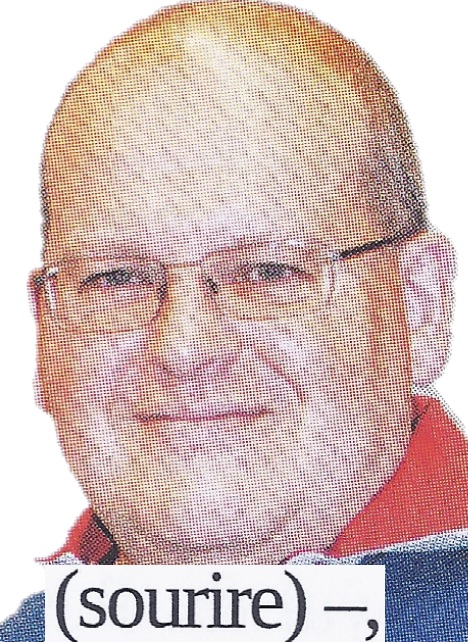
\includegraphics[height=1ex]{sourire.jpg}}
\setbeamertemplate{itemize item}[image]
\graphicspath{{../shared-resources/pictures/},{pictures/}}

% --------- PACKAGES FOR SCIENTIFIC WRITINGS ---------

\usepackage{amsmath}
\usepackage{stackengine}
\usepackage{siunitx}

\sisetup{detect-all}
\DeclareSIQualifier\peaktopeak{PP}
\DeclareSIUnit\voltptp{\volt\peaktopeak}
\DeclareSIUnit\au{a.u.}

\usepackage{pgfplots} % drawing graphs
\usepackage{empheq}
\pgfplotsset{width=\textwidth}

% --------- PACKAGES FOR REFERENCES AND BIBLIOGRAPHY ----------

\usepackage{hyperref}
\usepackage[
	backend=biber,
	style=alphabetic,
	citestyle=authoryear
]{biblatex}
\addbibresource{../shared-resources/biblio/biblio.bib}

% -------- Outline --------

\AtBeginSection[]
{
  \begin{frame}[noframenumbering]
  \frametitle{Outline}
  \tableofcontents[currentsection, hideothersubsections]
  \end{frame} 
}

% ------- Functions ----------

\renewcommand\epsilon{\varepsilon}

\newcommand{\op}[1]{\mathop{}\!\ensurestackMath{\smash{\stackon[-0.8ex]{%
    \mathbf{#1}}{\mathbf{\hat{}}}}}\vphantom{#1}} % used to display hat higher (look nicer)